\chapter{Скифы}
%\corner{64}
\vepsianrose

\diagdash Итак, парни! Сегодня у нас операция <<Прорыв>>.\mdash сообщил команде Адмирал за завтраком.

\diagdash Это что?

\diagdash Тут тема такая. Я начитался в инете, что у местных срывает крышу от жадности и желания денег из воздуха\mdash они организовали взимание платы за проход к палеовулкану со стороны автостоянки.

\diagdash !!!

\diagdash Именно. Поэтому, план <<А>>: оцениваем степень серьёзности охраны, делаем морду кирпичом и прём напролом, план <<Б>>: обходим кругом эту будку недовахтёров и~ломимся через лес напрямки.

\diagdash Дерзко, однако.

\diagdash Ну а фигли$\quldots$ %?$\ldots$?$\ldots$

%\vspace{1em}
\newpage

%\begin{wrapfigure}[18]{l}{0.5\textwidth}
\begin{figure}[h]
	\centering
	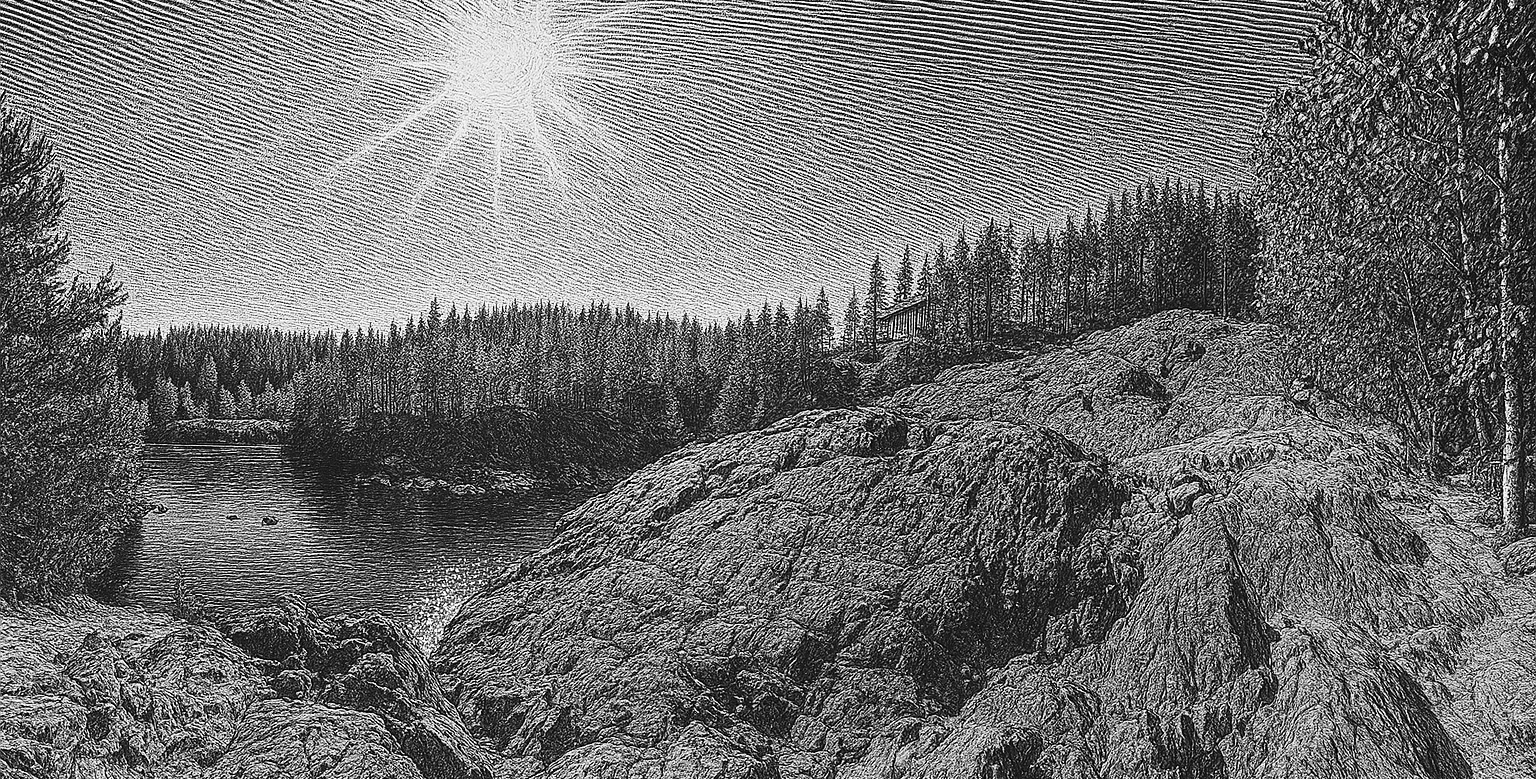
\includegraphics[width=1.0\textwidth]{58_1_vulkan}
	\caption{\small\textit{...Древний потухший вулкан спал беспробудным сном...}}
\end{figure}
%\end{wrapfigure}

$\ldots$Спустя полчаса они запарковались у палеовулкана и~успешно осуществили свой план <<А>>, оценив обстановку:

\diagdash А обратно выйдем лесом, нормальный ход,\mdash сообщил команде Адмирал,\mdash <<Да,~скифы\mdash мы! Да,~азиаты\mdash мы, c~раскосыми и~жадными очами!!!>>

\diagdash Ну ты даёшь, Шурик!

\diagdash Сам удивляюсь! Немного наглости и мы у цели. Ладно, пошли смотреть чего тут есть.

Скифы прошли к самому палеовулкану, аккуратно спускаясь по камням и узким тропкам. Древний потухший вулкан спал беспробудным сном, год за годом его размывали потоки Суны. Вид на долину был красив\mdash тут было раздвоение канала\mdash на одной протоке стояла гирвасская ГЭС, а~на~другой собственно и находился палеовулкан. Самой электростанции ребята так и~не~увидели поближе, вид на~неё~скрывала гора и~лес. 

%\begin{wrapfigure}[18]{l}{0.5\textwidth}
\begin{figure}[h]
	\centering
	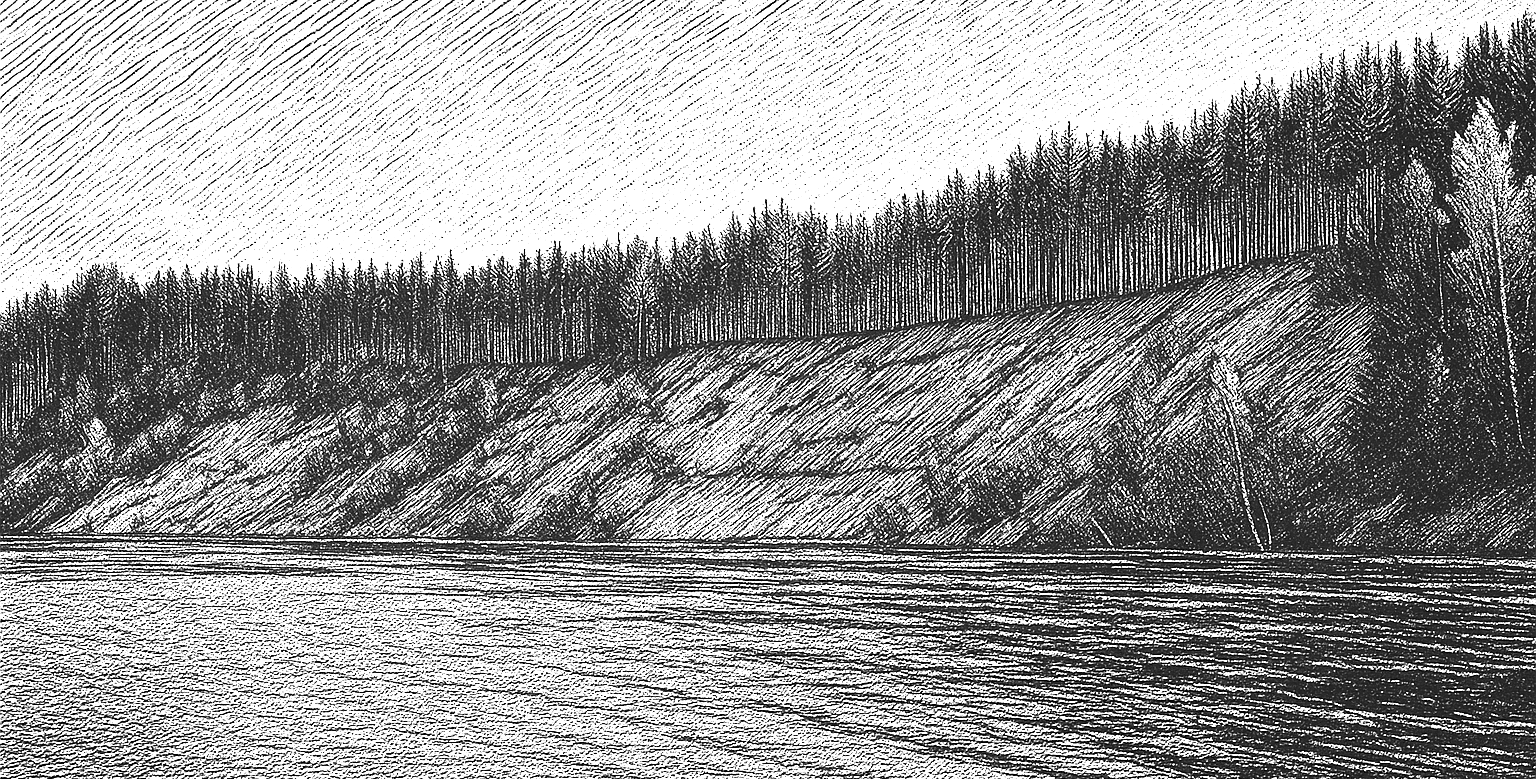
\includegraphics[width=1.0\textwidth]{57_obriv}
	\caption{\small\textit{...наверху обрыв сплошь порос высокими соснами...}}
\end{figure}
%\end{wrapfigure}

Команда спустилась в самый низ долины, к воде на~берег. Им предстал вид высоченного обрыва Пионерного канала. Наверху обрыв сплошь порос высокими соснами. Вид был что надо\mdash команда вдоволь нафотографировалась и~на~фоне обрыва, и~на~фоне вулкана и пошла потихоньку обратно.

\diagdash Куда теперь, Сусанин?\mdash ребята ждали, пока Адмрал тяжело поднимался по обрыву.

\diagdash Фух,\mdash отдышался Адмирал,\mdash теперь вон в лес сворачиваем, там просека должна быть\mdash по ней выйдем на~дорогу.

\diagdash Партизанен, блин!\mdash Паша пошёл вперёд, остальные стали подтягиваться.

\diagdash Нормалёк, мы не ищем лёгких путей, ну?

%%\begin{wrapfigure}[18]{l}{0.5\textwidth}
%	\begin{figure}[h]
%	\centering
%	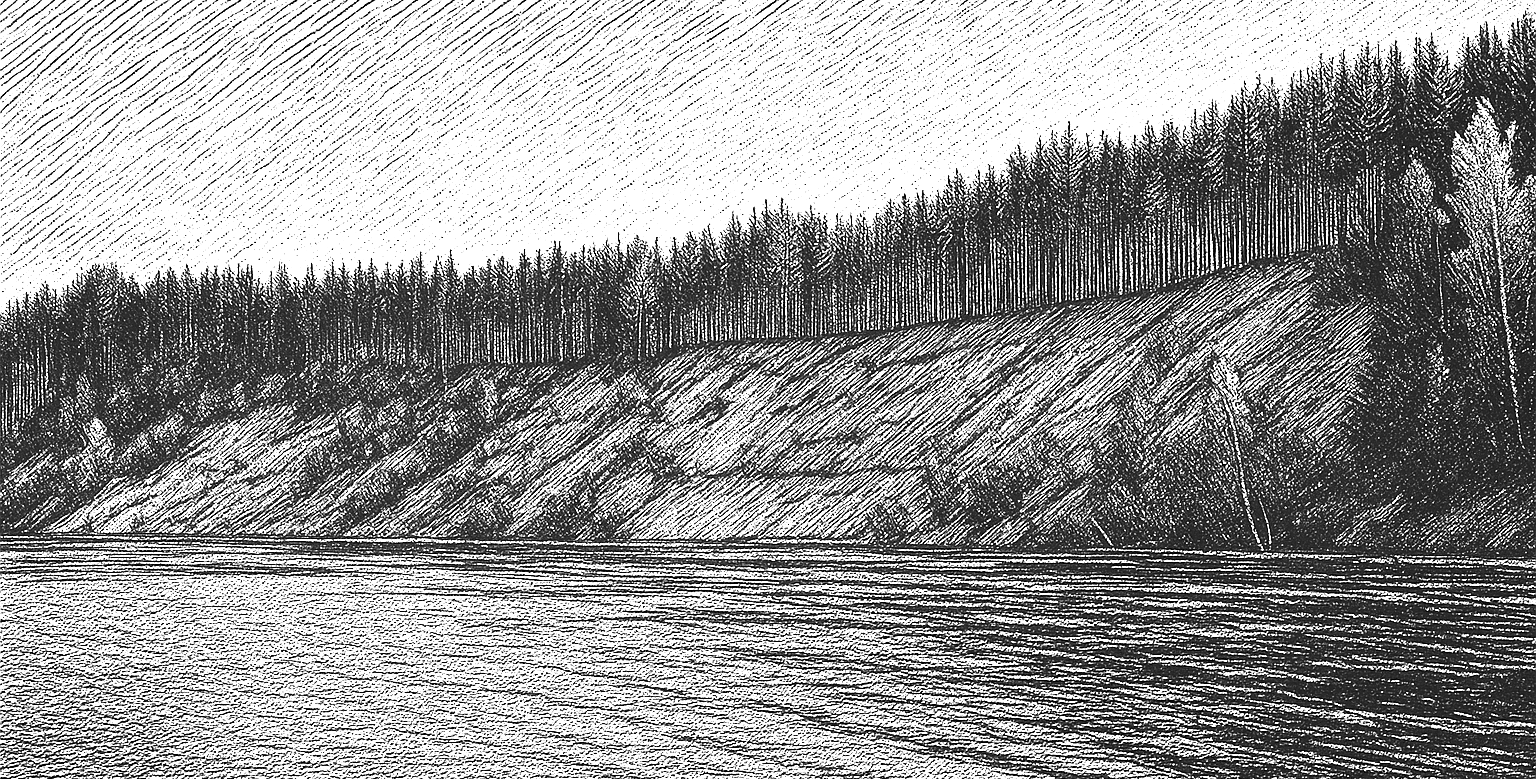
\includegraphics[width=1.0\textwidth]{57_obriv}
%	\caption{\small\textit{...наверху обрыв сплошь порос высокими соснами...}}
%	\end{figure}
%%\end{wrapfigure}

Вскоре ребята выбрались по просеке из леса и~дотопали до своих машин, накупив в лавочках всяких сувенирных безделушек\mdash магнитов на холодильник и~прочего. Настала~пора~прощаться:

\diagdash Ну, парни, дальше наши пути расходятся.\mdash Адмирал с грустью опёрся на дверь своего авто.

\diagdash Да, мы кочуем на Белозёрск, нам ещё на паром успеть надо.\mdash Серёга решил дополнить путешествие таким своеобразным аккордом.

\diagdash Скифы, ничего не попишешь!\mdash подыграл Замполит, и все заржали.

\diagdash Что есть, то есть! 

\diagdash А мы до Новгорода\mdash там заночуем, и уже до Москвы завтра. Удачи вам, парни, и хорошей дороги!\mdash Адмирал, Замполит и Паша попрощались с Серёгой и Русланом. Команда разделилась$\ldots$

%\vspace{1em}

$\ldots$Шурик гнал своё авто по узким пустынным карельским дорогам, упиваясь красотой местных пейзажей\mdash скальные выходы породы, высокий корабельный лес, облачное низкое небо. Уезжать, понятно, ему не~хотелось. Он бы с удовольствием пожил тут с полгодика, думалось ему$\ldots$ Тем временем, карельская погода провожала их в~своей манере\mdash резко потемнело и пошёл дождь, трасса намокла:

{
\diagdash Шурик, мож не будем так гнать?\mdash отвлёкся Замполит от телефона\mdash его уже вовсю беспокоили звонками по работе.

\diagdash М? Ну ладно, оторвёмся завтра на М\sdash11.\mdash согласился Адмирал и сел на хвост какой\sdash то фуре, сбавив обороты. Паша на заднем сиденье прикорнул, Замполит тоже прислонился к двери и закемарил.
}

\newpage

%\begin{wrapfigure}[18]{l}{0.5\textwidth}
\begin{figure}[h]
	\centering
	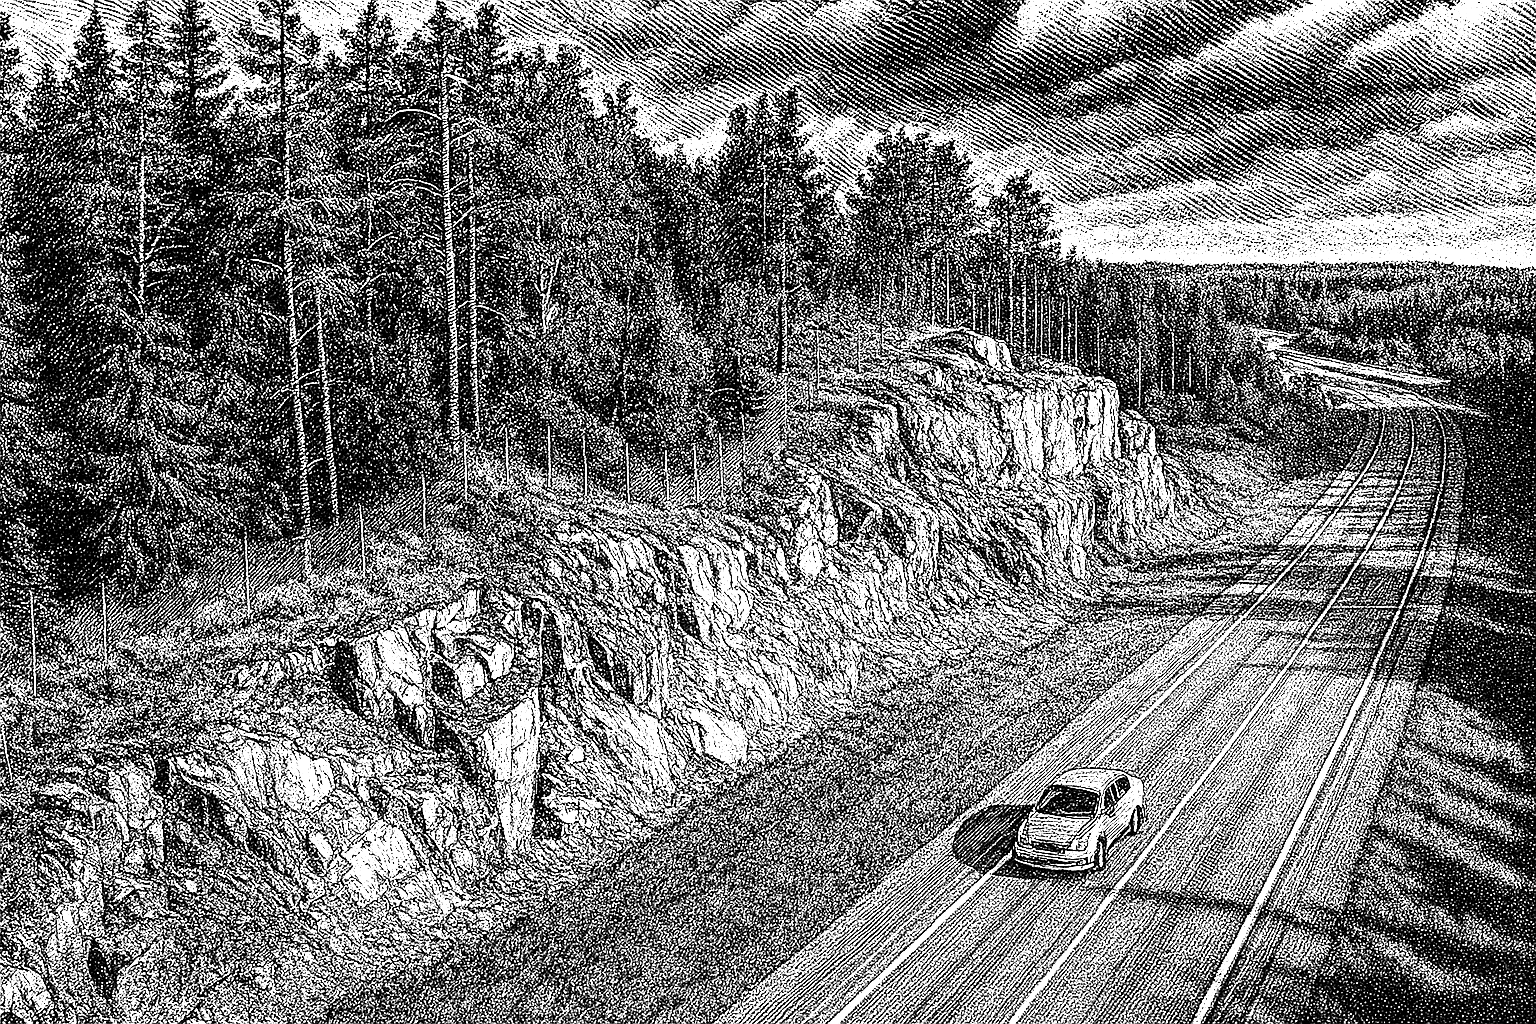
\includegraphics[width=1.0\textwidth]{59_1_avto}
	\caption{\small\textit{...упиваясь красотой местных пейзажей...}}
\end{figure}
%\end{wrapfigure}
Туристы\sdash водники возвращались домой. Настроение у~Адмирала было сквернейшее\mdash мало того, что он быстро устал от~трассы, дороги, так и~покидать Карелию не~хотелось а\sdash а\sdash абсолютно\mdash сердцем он был весь там, на~каменистых берегах с~упоительно красивыми янтарными соснами. В~соответствии с~настроением из~колонок его авто лился бессмертный вокал Дио и~завывала гитара Блэкмора:

\vspace{1.0cm}
\noindent\textit{%
	\hspace*{3.4cm}$\ldots$I'm going home\\
	\hspace*{3.4cm}My eyes are bleeding\\
	\hspace*{3.4cm}And my heart is leaving here$\ldots$%\\
%	\hspace*{3.4cm}The place I've known\\
%	\hspace*{3.4cm}But it's not home\\
%	\hspace*{3.4cm}O-о-оh$\exldotsit$\\%!$\ldots$\\
%	\hspace*{3.4cm}Take me back, take me back\\
%	\hspace*{3.4cm}Back to my home ooh, ooh, ooh
}

{\raggedleft \scriptsize \mdash Stargazer, гр. Rainbow. \par}

%\vspace{0.47cm} 

\newpage
$\ldots$Часам к девяти вечера парни добрались до~гостиницы в~Новгороде и заночевали там, естественно, предварительно совершив набег на~местный магазинчик под~предводительством Замполита. Заселившись, они выползли к крылечку на лавочки и~открыли по~баночке пенного. Каждый залип в~мобильник, общаясь с~роднёй, цивилизация. 

Шурик вдруг ощутил себя прежним, больше не~Адмиралом Сплава. И~Киря, уже всю дорогу деловито обсуждающий по~телефону что\sdash то по~бизнес\sdash вопросам, уже больше не~Замполит, а~прежний делец Киря. Да~и~Пашка больше не~Рыбак и~Вперёдсмотрящий. Словом, они неумолимо возвращались обратно в прежнюю жизнь, как бы ни хотел Шурик продлить это отрешённое ото~всего состояние$\ldots$

$\ldots$На следующий день парни откопали в Новгороде очень приличную столовую при каком\sdash то заводе и, позавтракав, двинули в путь. Скоростная М\sdash 11 до Москвы пролетела почти как одно мгновение, прерванное только автозаправкой где\sdash то в районе Твери.

Шурик развёз товарищей по домам\mdash сначала забросили Пашу, а~затем двинули вместе с~Кирей на~свой восток Москвы по МКАДу. Привычный дорожный траффик, пробки, суета. Как разительно это отличалось от того, что буквально пару дней назад было у них: спокойствие, пение птиц, шум ветра в чистейших карельских хвойных лесах. Забросив и Кирю, Шурик наконец добрался до дома\mdash уставший от дороги, но очень счастливый, что пережил эти две безумно насыщенные приключениями недели.





%$\ldots$Парни добрались до Новгорода часам к девяти вечера и  через вечерние пробки просочились к гостинице на окраине:
%
%\diagdash Шурик, я там магазинчик заприметил, когда мы поворачивали сюда.\mdash недвусмысленно намекнул Замполит.
%
%\diagdash Парни, давайте сначала заселимся?\mdash Адмирал вылез из авто и размял спину.
%
%Они заселились в небольшой номер, где было 2 кровати и диван:
%
%\diagdash Так, кому диван\mdash тянем на спичках.
%
%\diagdash Ой, ну вас, я на диване, только пошли быстрее в~магаз?\mdash сдался без боя Замполит.


%\vspace{1em}

\begin{center}
	\psvectorian[scale=0.4]{88} % Красивый вензелёк :)
\end{center}
